% Options for packages loaded elsewhere
\PassOptionsToPackage{unicode}{hyperref}
\PassOptionsToPackage{hyphens}{url}
%
\documentclass[
]{article}
\usepackage{lmodern}
\usepackage{amssymb,amsmath}
\usepackage{ifxetex,ifluatex}
\ifnum 0\ifxetex 1\fi\ifluatex 1\fi=0 % if pdftex
  \usepackage[T1]{fontenc}
  \usepackage[utf8]{inputenc}
  \usepackage{textcomp} % provide euro and other symbols
\else % if luatex or xetex
  \usepackage{unicode-math}
  \defaultfontfeatures{Scale=MatchLowercase}
  \defaultfontfeatures[\rmfamily]{Ligatures=TeX,Scale=1}
\fi
% Use upquote if available, for straight quotes in verbatim environments
\IfFileExists{upquote.sty}{\usepackage{upquote}}{}
\IfFileExists{microtype.sty}{% use microtype if available
  \usepackage[]{microtype}
  \UseMicrotypeSet[protrusion]{basicmath} % disable protrusion for tt fonts
}{}
\makeatletter
\@ifundefined{KOMAClassName}{% if non-KOMA class
  \IfFileExists{parskip.sty}{%
    \usepackage{parskip}
  }{% else
    \setlength{\parindent}{0pt}
    \setlength{\parskip}{6pt plus 2pt minus 1pt}}
}{% if KOMA class
  \KOMAoptions{parskip=half}}
\makeatother
\usepackage{xcolor}
\IfFileExists{xurl.sty}{\usepackage{xurl}}{} % add URL line breaks if available
\IfFileExists{bookmark.sty}{\usepackage{bookmark}}{\usepackage{hyperref}}
\hypersetup{
  pdftitle={R Notebook},
  hidelinks,
  pdfcreator={LaTeX via pandoc}}
\urlstyle{same} % disable monospaced font for URLs
\usepackage[margin=1in]{geometry}
\usepackage{color}
\usepackage{fancyvrb}
\newcommand{\VerbBar}{|}
\newcommand{\VERB}{\Verb[commandchars=\\\{\}]}
\DefineVerbatimEnvironment{Highlighting}{Verbatim}{commandchars=\\\{\}}
% Add ',fontsize=\small' for more characters per line
\usepackage{framed}
\definecolor{shadecolor}{RGB}{248,248,248}
\newenvironment{Shaded}{\begin{snugshade}}{\end{snugshade}}
\newcommand{\AlertTok}[1]{\textcolor[rgb]{0.94,0.16,0.16}{#1}}
\newcommand{\AnnotationTok}[1]{\textcolor[rgb]{0.56,0.35,0.01}{\textbf{\textit{#1}}}}
\newcommand{\AttributeTok}[1]{\textcolor[rgb]{0.77,0.63,0.00}{#1}}
\newcommand{\BaseNTok}[1]{\textcolor[rgb]{0.00,0.00,0.81}{#1}}
\newcommand{\BuiltInTok}[1]{#1}
\newcommand{\CharTok}[1]{\textcolor[rgb]{0.31,0.60,0.02}{#1}}
\newcommand{\CommentTok}[1]{\textcolor[rgb]{0.56,0.35,0.01}{\textit{#1}}}
\newcommand{\CommentVarTok}[1]{\textcolor[rgb]{0.56,0.35,0.01}{\textbf{\textit{#1}}}}
\newcommand{\ConstantTok}[1]{\textcolor[rgb]{0.00,0.00,0.00}{#1}}
\newcommand{\ControlFlowTok}[1]{\textcolor[rgb]{0.13,0.29,0.53}{\textbf{#1}}}
\newcommand{\DataTypeTok}[1]{\textcolor[rgb]{0.13,0.29,0.53}{#1}}
\newcommand{\DecValTok}[1]{\textcolor[rgb]{0.00,0.00,0.81}{#1}}
\newcommand{\DocumentationTok}[1]{\textcolor[rgb]{0.56,0.35,0.01}{\textbf{\textit{#1}}}}
\newcommand{\ErrorTok}[1]{\textcolor[rgb]{0.64,0.00,0.00}{\textbf{#1}}}
\newcommand{\ExtensionTok}[1]{#1}
\newcommand{\FloatTok}[1]{\textcolor[rgb]{0.00,0.00,0.81}{#1}}
\newcommand{\FunctionTok}[1]{\textcolor[rgb]{0.00,0.00,0.00}{#1}}
\newcommand{\ImportTok}[1]{#1}
\newcommand{\InformationTok}[1]{\textcolor[rgb]{0.56,0.35,0.01}{\textbf{\textit{#1}}}}
\newcommand{\KeywordTok}[1]{\textcolor[rgb]{0.13,0.29,0.53}{\textbf{#1}}}
\newcommand{\NormalTok}[1]{#1}
\newcommand{\OperatorTok}[1]{\textcolor[rgb]{0.81,0.36,0.00}{\textbf{#1}}}
\newcommand{\OtherTok}[1]{\textcolor[rgb]{0.56,0.35,0.01}{#1}}
\newcommand{\PreprocessorTok}[1]{\textcolor[rgb]{0.56,0.35,0.01}{\textit{#1}}}
\newcommand{\RegionMarkerTok}[1]{#1}
\newcommand{\SpecialCharTok}[1]{\textcolor[rgb]{0.00,0.00,0.00}{#1}}
\newcommand{\SpecialStringTok}[1]{\textcolor[rgb]{0.31,0.60,0.02}{#1}}
\newcommand{\StringTok}[1]{\textcolor[rgb]{0.31,0.60,0.02}{#1}}
\newcommand{\VariableTok}[1]{\textcolor[rgb]{0.00,0.00,0.00}{#1}}
\newcommand{\VerbatimStringTok}[1]{\textcolor[rgb]{0.31,0.60,0.02}{#1}}
\newcommand{\WarningTok}[1]{\textcolor[rgb]{0.56,0.35,0.01}{\textbf{\textit{#1}}}}
\usepackage{graphicx,grffile}
\makeatletter
\def\maxwidth{\ifdim\Gin@nat@width>\linewidth\linewidth\else\Gin@nat@width\fi}
\def\maxheight{\ifdim\Gin@nat@height>\textheight\textheight\else\Gin@nat@height\fi}
\makeatother
% Scale images if necessary, so that they will not overflow the page
% margins by default, and it is still possible to overwrite the defaults
% using explicit options in \includegraphics[width, height, ...]{}
\setkeys{Gin}{width=\maxwidth,height=\maxheight,keepaspectratio}
% Set default figure placement to htbp
\makeatletter
\def\fps@figure{htbp}
\makeatother
\setlength{\emergencystretch}{3em} % prevent overfull lines
\providecommand{\tightlist}{%
  \setlength{\itemsep}{0pt}\setlength{\parskip}{0pt}}
\setcounter{secnumdepth}{-\maxdimen} % remove section numbering

\title{R Notebook}
\author{}
\date{\vspace{-2.5em}}

\begin{document}
\maketitle

\hypertarget{authors}{%
\subsubsection{Authors:}\label{authors}}

\begin{itemize}
\tightlist
\item
  Simin Zhang
\item
  Yiman Liu
\item
  Zhi Wen
\end{itemize}

\hypertarget{tasks}{%
\section{Tasks}\label{tasks}}

\begin{enumerate}
\def\labelenumi{\arabic{enumi}.}
\tightlist
\item
  (10 pts / 1 hr) Install MySQL using the instructions provided in the
  practicum.
\end{enumerate}

\begin{enumerate}
\def\labelenumi{\arabic{enumi}.}
\setcounter{enumi}{1}
\tightlist
\item
  (10 pts / 2 hrs) Create an R or Jupyter Notebook.
\end{enumerate}

\begin{enumerate}
\def\labelenumi{\arabic{enumi}.}
\setcounter{enumi}{2}
\tightlist
\item
  (10 pts / 2 hrs) Analyze the problem of contact tracing and create a
  conceptual model in UML.
\end{enumerate}

\begin{enumerate}
\def\labelenumi{\arabic{enumi}.}
\setcounter{enumi}{3}
\tightlist
\item
  (10 pts / 1 hr) From the Conceptual Model, construct a logical data
  model expressed as an ERD using IE (Crow's Foot) and a tool of your
  choice that is in at least BCNF.
\end{enumerate}

\begin{itemize}
\tightlist
\item
  ERD \& URL to its LucidChart diagram:
  \url{https://lucid.app/lucidchart/614f280e-f6d6-4a87-bd82-e9b3a1f8f161/edit?page=0_0\#?folder_id=home\&browser=icon}
\end{itemize}

\begin{itemize}
\tightlist
\item
  Using functional dependencies, show that the schema in in at least
  BCNF
\end{itemize}

\begin{verbatim}
[Person]

PersonId: single valued
EmployeeId: single valued
FirstName: single valued
LastName: single valued
DOB: single valued
Gender: single valued
Address: single valued
City: single valued
State: single valued
Phone: single valued
Email: single valued
SMS: single valued
DateOfStartQuarantine: single valued
1NF ✔️

(key)A: PersonId
(non-key)B: EmployeeId
(non-key)C: FirstName
(non-key)D: LastName
(non-key)E: DOB
(non-key)F: Gender
(non-key)G: Address
(non-key)H: City
(non-key)I: State
(non-key)J: Phone
(non-key)K: Email
(non-key)L: SMS
(non-key)M: DateOfStartQuarantine

A -> B
A -> C
A -> D
A -> E
A -> F
A -> G
A -> H
A -> I
A -> J
A -> K
A -> L
A -> M
2NF ✔️

No non-key attribute can decide A(key), so BCNF ✔️

[MedicalProvider]

MedicalProviderId: single valued
Title: single valued
FirstName: single valued
LastName: single valued
PersonId: single valued
1NF ✔️

(key)A: MedicalProviderId
(non-key)B: Title
(non-key)C: FirstName
(non-key)D: LastName
(non-key)E: PersonId

A -> B
A -> C
A -> D
A -> E
2NF ✔️

No non-key attribute can decide A(key), so BCNF ✔️

[Hospital]

HospitalId: single valued
Name: single valued
Address: single valued
Phone: single valued
1NF ✔️

(key)A: HospitalId
(non-key)B: Name
(non-key)C: Address
(non-key)D: Phone

A -> B
A -> C
A -> D
2NF ✔️

No non-key attribute can decide A(key), so BCNF ✔️

[Symptom]

SymptomId: single valued
ReportId: single valued
DateOfSymptomOnset: single valued
SymptomDetail: single valued
1NF ✔️

(key)A: SymptomId
(non-key)B: ReportId
(non-key)C: DateOfSymptomOnset
(non-key)D: SymptomDetail

A -> B
A -> C
A -> D
2NF ✔️

No non-key attribute can decide A(key), so BCNF ✔️

[SelfReport]

ReportId: single valued
PersonId: single valued
ReportDate:  single valued
Detail: single valued
Temperature: single valued
ProtectiveBehavior: single valued
Quarantined: single valued
1NF ✔️

(key)A: ReportId
(non-key)B: PersonId
(non-key)C: ReportDate
(non-key)D: Detail
(non-key)E: Temperature
(non-key)F: ProtectiveBehavior
(non-key)G: Quarantined

A -> B
A -> C
A -> D
A -> E
A -> F
A -> G
2NF ✔️

No non-key attribute can decide A(key), so BCNF ✔️

[TestResult]

TestResultId: single valued
ReportId: single valued
Description: single valued
Positive: single valued

(key)A: TestResultId
(non-key)B: ReportId
(non-key)C: Description
(non-key)D: Positive

A -> B
A -> C
A -> D
2NF ✔️

No non-key attribute can decide A(key), so BCNF ✔️

[Employee]

EmployeeId: single valued
FirstName: single valued
LastName: single valued
Phone: single valued
1NF ✔️

(key)A: EmployeeId
(non-key)B: FirstName
(non-key)C: LastName
(non-key)D: Phone

A -> B
A -> C
A -> D
2NF ✔️

No non-key attribute can decide A(key), so BCNF ✔️

[Event]

EventId: single valued
EventDate: single valued
Address: single valued
City: single valued
State: single valued
Detail: single valued
1NF ✔️

(key)A: EventId
(non-key)B: EventDate
(non-key)C: Address
(non-key)D: City
(non-key)E: State
(non-key)F: Detail

A -> B
A -> C
A -> D
A -> E
A -> F
2NF ✔️

No non-key attribute can decide A(key), so BCNF ✔️

[SupportiveServices]

SupportiveServicesId: single valued
Title: single valued
PersonId: single valued
1NF ✔️

(key)A: SupportiveServicesId
(non-key)B: Title
(non-key)C: PersonId

A -> B
A -> C
2NF ✔️

No non-key attribute can decide A(key), so BCNF ✔️

[Notification]

NotificationId: single valued
PersonId: single valued
NotificationType: single valued
NotificationDate: single valued
Detail: single valued
1NF ✔️

(key)A: NotificationId
(non-key)B: PersonId
(non-key)C: NotificationType
(non-key)D: NotificationDate
(non-key)E: Detail

A -> B
A -> C
A -> D
A -> E
2NF ✔️

No non-key attribute can decide A(key), so BCNF ✔️
\end{verbatim}

\begin{enumerate}
\def\labelenumi{\arabic{enumi}.}
\setcounter{enumi}{4}
\tightlist
\item
  (20 pts / 1.5 hrs) Create a set of SQL data definition statements,
  realize that schema in MySQL by executing the script from the MySQL
  console.
\end{enumerate}

\begin{Shaded}
\begin{Highlighting}[]
\KeywordTok{CREATE} \KeywordTok{TABLE}\NormalTok{ Hospital (}
\NormalTok{  HospitalId }\DataTypeTok{INT} \KeywordTok{NOT} \KeywordTok{NULL}\NormalTok{,}
\NormalTok{  Name }\DataTypeTok{VARCHAR}\NormalTok{(}\DecValTok{45}\NormalTok{),}
\NormalTok{  Address }\DataTypeTok{VARCHAR}\NormalTok{(}\DecValTok{45}\NormalTok{),}
\NormalTok{  Phone }\DataTypeTok{VARCHAR}\NormalTok{(}\DecValTok{20}\NormalTok{),}
  \KeywordTok{PRIMARY} \KeywordTok{KEY}\NormalTok{ (HospitalId)}
\NormalTok{)}
\KeywordTok{COMMENT} \OperatorTok{=} \StringTok{'Health center for connecting with patients and contacts.'}\NormalTok{;}


\KeywordTok{CREATE} \KeywordTok{TABLE}\NormalTok{ MedicalProvider (}
\NormalTok{  MedicalProviderId }\DataTypeTok{INT} \KeywordTok{NOT} \KeywordTok{NULL}\NormalTok{,}
\NormalTok{  Title }\DataTypeTok{VARCHAR}\NormalTok{(}\DecValTok{20}\NormalTok{),}
\NormalTok{  FirstName }\DataTypeTok{VARCHAR}\NormalTok{(}\DecValTok{20}\NormalTok{),}
\NormalTok{  LastName }\DataTypeTok{VARCHAR}\NormalTok{(}\DecValTok{20}\NormalTok{),}
\NormalTok{  HospitalId }\DataTypeTok{INT} \KeywordTok{NOT} \KeywordTok{NULL}\NormalTok{,}
  \KeywordTok{PRIMARY} \KeywordTok{KEY}\NormalTok{ (MedicalProviderId),}
  \KeywordTok{FOREIGN} \KeywordTok{KEY}\NormalTok{ (HospitalId)}
    \KeywordTok{REFERENCES}\NormalTok{ Hospital(HospitalId)}
\NormalTok{)}
\KeywordTok{COMMENT} \OperatorTok{=} \StringTok{'Doctor who diagnosis patients.'}\NormalTok{;}


\KeywordTok{CREATE} \KeywordTok{TABLE}\NormalTok{ Employee (}
\NormalTok{  EmployeeId }\DataTypeTok{INT} \KeywordTok{NOT} \KeywordTok{NULL}\NormalTok{,}
\NormalTok{  FirstName }\DataTypeTok{VARCHAR}\NormalTok{(}\DecValTok{20}\NormalTok{),}
\NormalTok{  LastName }\DataTypeTok{VARCHAR}\NormalTok{(}\DecValTok{20}\NormalTok{),}
\NormalTok{  Phone }\DataTypeTok{INT}\NormalTok{,}
  \KeywordTok{PRIMARY} \KeywordTok{KEY}\NormalTok{ (EmployeeId)}
\NormalTok{)}
\KeywordTok{COMMENT} \OperatorTok{=} \StringTok{'Employee from health department who is responsible for contacting patients and contact.'}\NormalTok{;}


\KeywordTok{CREATE} \KeywordTok{TABLE}\NormalTok{ Person (}
\NormalTok{  PersonId }\DataTypeTok{INT} \KeywordTok{NOT} \KeywordTok{NULL}\NormalTok{,}
\NormalTok{  MedicalProviderId }\DataTypeTok{INT}\NormalTok{,}
\NormalTok{  EmployeeId }\DataTypeTok{INT} \KeywordTok{NOT} \KeywordTok{NULL}\NormalTok{,}
\NormalTok{  FirstName }\DataTypeTok{VARCHAR}\NormalTok{(}\DecValTok{20}\NormalTok{),}
\NormalTok{  LastName }\DataTypeTok{VARCHAR}\NormalTok{(}\DecValTok{20}\NormalTok{),}
\NormalTok{  DOB }\DataTypeTok{DATE}\NormalTok{,}
\NormalTok{  Gender ENUM(}\StringTok{'male'}\NormalTok{, }\StringTok{'female'}\NormalTok{),}
\NormalTok{  Address }\DataTypeTok{VARCHAR}\NormalTok{(}\DecValTok{45}\NormalTok{),}
\NormalTok{  City }\DataTypeTok{VARCHAR}\NormalTok{(}\DecValTok{45}\NormalTok{),}
\NormalTok{  State }\DataTypeTok{VARCHAR}\NormalTok{(}\DecValTok{45}\NormalTok{),}
\NormalTok{  Phone }\DataTypeTok{VARCHAR}\NormalTok{(}\DecValTok{45}\NormalTok{),}
\NormalTok{  Email }\DataTypeTok{VARCHAR}\NormalTok{(}\DecValTok{45}\NormalTok{),}
\NormalTok{  SMS }\DataTypeTok{VARCHAR}\NormalTok{(}\DecValTok{45}\NormalTok{),}
\NormalTok{  DateOfStartQuarantine }\DataTypeTok{DATE}\NormalTok{,}
\NormalTok{  SourceOfInfection }\DataTypeTok{VARCHAR}\NormalTok{(}\DecValTok{45}\NormalTok{),}
\NormalTok{  RiskLevel }\DataTypeTok{INT}\NormalTok{,}
  \KeywordTok{PRIMARY} \KeywordTok{KEY}\NormalTok{ (PersonId),}
  \KeywordTok{FOREIGN} \KeywordTok{KEY}\NormalTok{ (MedicalProviderId)}
    \KeywordTok{REFERENCES}\NormalTok{ MedicalProvider(MedicalProviderId),}
  \KeywordTok{FOREIGN} \KeywordTok{KEY}\NormalTok{ (EmployeeId)}
    \KeywordTok{REFERENCES}\NormalTok{ Employee(EmployeeId)}
\NormalTok{)}
\KeywordTok{COMMENT} \OperatorTok{=} \StringTok{'Either a test positive patient or a potiential patient who contacts with a patient'}\NormalTok{;}


\KeywordTok{CREATE} \KeywordTok{TABLE}\NormalTok{ Notification (}
\NormalTok{  NotificationId }\DataTypeTok{INT} \KeywordTok{NOT} \KeywordTok{NULL}\NormalTok{,}
\NormalTok{  PersonId }\DataTypeTok{INT} \KeywordTok{NOT} \KeywordTok{NULL}\NormalTok{,}
\NormalTok{  NotificationType }\DataTypeTok{VARCHAR}\NormalTok{(}\DecValTok{45}\NormalTok{),}
\NormalTok{  NotificationDate }\DataTypeTok{DATE}\NormalTok{,}
\NormalTok{  Detail }\DataTypeTok{VARCHAR}\NormalTok{(}\DecValTok{45}\NormalTok{),}
  \KeywordTok{PRIMARY} \KeywordTok{KEY}\NormalTok{ (NotificationId),}
  \KeywordTok{FOREIGN} \KeywordTok{KEY}\NormalTok{ (PersonId)}
    \KeywordTok{REFERENCES}\NormalTok{ Person (PersonId)}
\NormalTok{)}
\KeywordTok{COMMENT} \OperatorTok{=} \StringTok{'Both patients and contacts will receive notification based on their health condition.'}\NormalTok{;}


\KeywordTok{CREATE} \KeywordTok{TABLE}\NormalTok{ Event (}
\NormalTok{  EventId }\DataTypeTok{INT} \KeywordTok{NOT} \KeywordTok{NULL}\NormalTok{,}
\NormalTok{  EventDate }\DataTypeTok{DATE}\NormalTok{,}
\NormalTok{  Address }\DataTypeTok{VARCHAR}\NormalTok{(}\DecValTok{45}\NormalTok{),}
\NormalTok{  City }\DataTypeTok{VARCHAR}\NormalTok{(}\DecValTok{45}\NormalTok{),}
\NormalTok{  State }\DataTypeTok{VARCHAR}\NormalTok{(}\DecValTok{45}\NormalTok{),}
\NormalTok{  Detail }\DataTypeTok{VARCHAR}\NormalTok{(}\DecValTok{45}\NormalTok{),}
  \KeywordTok{PRIMARY} \KeywordTok{KEY}\NormalTok{ (EventId)}
\NormalTok{)}
\KeywordTok{COMMENT} \OperatorTok{=} \StringTok{'The event that patients and contacts attend.'}\NormalTok{;}


\KeywordTok{CREATE} \KeywordTok{TABLE}\NormalTok{ PersonEvent (}
\NormalTok{  PersonId }\DataTypeTok{INT} \KeywordTok{NOT} \KeywordTok{NULL}\NormalTok{,}
\NormalTok{  EventId }\DataTypeTok{INT} \KeywordTok{NOT} \KeywordTok{NULL}\NormalTok{,}
  \KeywordTok{PRIMARY} \KeywordTok{KEY}\NormalTok{ (PersonId, EventId),}
  \KeywordTok{FOREIGN} \KeywordTok{KEY}\NormalTok{ (PersonId)}
    \KeywordTok{REFERENCES}\NormalTok{ Person(PersonId),}
  \KeywordTok{FOREIGN} \KeywordTok{KEY}\NormalTok{ (EventId)}
    \KeywordTok{REFERENCES}\NormalTok{ Event(EventId)}
\NormalTok{);}


\KeywordTok{CREATE} \KeywordTok{TABLE}\NormalTok{ SupportiveServices (}
\NormalTok{  SupportiveServicesId }\DataTypeTok{INT} \KeywordTok{NOT} \KeywordTok{NULL}\NormalTok{,}
\NormalTok{  Title }\DataTypeTok{VARCHAR}\NormalTok{(}\DecValTok{45}\NormalTok{),}
  \KeywordTok{PRIMARY} \KeywordTok{KEY}\NormalTok{ (SupportiveServicesId)}
\NormalTok{)}
\KeywordTok{COMMENT} \OperatorTok{=} \StringTok{'Both patients and contacts will get support services during their quarantine if they face any inconvenience.'}\NormalTok{;}


\KeywordTok{CREATE} \KeywordTok{TABLE}\NormalTok{ ServicesPerson (}
\NormalTok{  SupportiveServicesId }\DataTypeTok{INT} \KeywordTok{NOT} \KeywordTok{NULL}\NormalTok{,}
\NormalTok{  PersonId }\DataTypeTok{INT} \KeywordTok{NOT} \KeywordTok{NULL}\NormalTok{,}
  \KeywordTok{PRIMARY} \KeywordTok{KEY}\NormalTok{ (SupportiveServicesId, PersonId),}
  \KeywordTok{FOREIGN} \KeywordTok{KEY}\NormalTok{ (SupportiveServicesId)}
    \KeywordTok{REFERENCES}\NormalTok{ SupportiveServices(SupportiveServicesId),}
  \KeywordTok{FOREIGN} \KeywordTok{KEY}\NormalTok{ (PersonId)}
    \KeywordTok{REFERENCES}\NormalTok{ Person(PersonId)}
\NormalTok{);}


\KeywordTok{CREATE} \KeywordTok{TABLE}\NormalTok{ SelfReport (}
\NormalTok{  ReportId }\DataTypeTok{INT} \KeywordTok{NOT} \KeywordTok{NULL}\NormalTok{,}
\NormalTok{  PersonId }\DataTypeTok{INT} \KeywordTok{NOT} \KeywordTok{NULL}\NormalTok{,}
\NormalTok{  ReportDate }\DataTypeTok{DATE}\NormalTok{,}
\NormalTok{  Temperature }\DataTypeTok{INT}\NormalTok{,}
\NormalTok{  ProtectiveBehavior }\DataTypeTok{VARCHAR}\NormalTok{(}\DecValTok{45}\NormalTok{),}
\NormalTok{  Quarantined TINYINT,}
  \KeywordTok{PRIMARY} \KeywordTok{KEY}\NormalTok{ (ReportId),}
  \KeywordTok{FOREIGN} \KeywordTok{KEY}\NormalTok{ (PersonId)}
    \KeywordTok{REFERENCES}\NormalTok{ Person(PersonId)}
\NormalTok{)}
\KeywordTok{COMMENT} \OperatorTok{=} \StringTok{'Daily data report such as temperature data, contact data.'}\NormalTok{;}


\KeywordTok{CREATE} \KeywordTok{TABLE}\NormalTok{ TestResult (}
\NormalTok{  TestResultId }\DataTypeTok{INT} \KeywordTok{NOT} \KeywordTok{NULL}\NormalTok{,}
\NormalTok{  ReportId }\DataTypeTok{INT} \KeywordTok{NOT} \KeywordTok{NULL}\NormalTok{,}
\NormalTok{  Description }\DataTypeTok{VARCHAR}\NormalTok{(}\DecValTok{45}\NormalTok{),}
\NormalTok{  Positive TINYINT,}
  \KeywordTok{PRIMARY} \KeywordTok{KEY}\NormalTok{ (TestResultId),}
  \KeywordTok{FOREIGN} \KeywordTok{KEY}\NormalTok{ (ReportId)}
    \KeywordTok{REFERENCES}\NormalTok{ SelfReport(ReportId)}
\NormalTok{)}
\KeywordTok{COMMENT} \OperatorTok{=} \StringTok{'If the test result is positive, which means this patient / contacts is diagnosed with Covid-19.'}\NormalTok{;}


\KeywordTok{CREATE} \KeywordTok{TABLE}\NormalTok{ Symptom (}
\NormalTok{  SymptomId }\DataTypeTok{INT} \KeywordTok{NOT} \KeywordTok{NULL}\NormalTok{,}
\NormalTok{  ReportId }\DataTypeTok{INT} \KeywordTok{NOT} \KeywordTok{NULL}\NormalTok{,}
\NormalTok{  DateOfSymptomOnset }\DataTypeTok{DATE}\NormalTok{,}
\NormalTok{  SymptomDetail }\DataTypeTok{VARCHAR}\NormalTok{(}\DecValTok{45}\NormalTok{),}
  \KeywordTok{PRIMARY} \KeywordTok{KEY}\NormalTok{ (SymptomId),}
  \KeywordTok{FOREIGN} \KeywordTok{KEY}\NormalTok{ (ReportId)}
    \KeywordTok{REFERENCES}\NormalTok{ SelfReport(ReportId)}
\NormalTok{)}
\KeywordTok{COMMENT} \OperatorTok{=} \StringTok{'Symptom description.'}\NormalTok{;}
\end{Highlighting}
\end{Shaded}

\begin{itemize}
\tightlist
\item
  Table {[}Employee{]} successfully created
\end{itemize}

\begin{itemize}
\tightlist
\item
  Table {[}Event{]} successfully created
\end{itemize}

\begin{itemize}
\tightlist
\item
  Table {[}Hospital{]} successfully created
\end{itemize}

\begin{itemize}
\tightlist
\item
  Table {[}MedicalProvider{]} successfully created
\end{itemize}

\begin{itemize}
\tightlist
\item
  Table {[}Notification{]} successfully created
\end{itemize}

\begin{itemize}
\tightlist
\item
  Table {[}Person{]} successfully created
\end{itemize}

\begin{itemize}
\tightlist
\item
  Table {[}PersonEvent{]} successfully created
\end{itemize}

\begin{itemize}
\tightlist
\item
  Table {[}SelfReport{]} successfully created
\end{itemize}

\begin{itemize}
\tightlist
\item
  Table {[}ServicesPerson{]} successfully created
\end{itemize}

\begin{itemize}
\tightlist
\item
  Table {[}SupportiveServices{]} successfully created
\end{itemize}

\begin{itemize}
\tightlist
\item
  Table {[}Symptom{]} successfully created
\end{itemize}

\begin{itemize}
\tightlist
\item
  Table {[}TestResult{]} successfully created
\end{itemize}

\begin{enumerate}
\def\labelenumi{\arabic{enumi}.}
\setcounter{enumi}{5}
\tightlist
\item
  (20 pts / 2 hrs) Work as a group to populate the tables with test
  data.
\end{enumerate}

\begin{enumerate}
\def\labelenumi{\arabic{enumi}.}
\setcounter{enumi}{6}
\tightlist
\item
  (20 pts / 1 hrs) Define and execute at least five queries that
  demonstrate that your database is working.
\end{enumerate}

\begin{Shaded}
\begin{Highlighting}[]
\CommentTok{-- Query 1: find the names and addresses of hospital which have more than 5 person and how much persons they have.}
\CommentTok{-- a join of at least three tables}
\CommentTok{-- a group by with a having clause}
\KeywordTok{SELECT}
\NormalTok{  h.Name,}
\NormalTok{  h.Address,}
  \FunctionTok{COUNT}\NormalTok{(p.PersonId) personCount}
\KeywordTok{FROM}\NormalTok{ Hospital h}
\KeywordTok{JOIN}\NormalTok{ MedicalProvider m}
\KeywordTok{ON}\NormalTok{ m.HospitalId}\OperatorTok{=}\NormalTok{h.HospitalId}
\KeywordTok{JOIN}\NormalTok{ Person p}
\KeywordTok{ON}\NormalTok{ p.MedicalProviderId}\OperatorTok{=}\NormalTok{m.MedicalProviderId}
\KeywordTok{GROUP} \KeywordTok{BY}\NormalTok{ h.name}
\KeywordTok{HAVING}\NormalTok{ personCount}\OperatorTok{>}\DecValTok{5}\NormalTok{;}




\CommentTok{-- Query 2: find the numbers of male and female persons.}
\CommentTok{-- an advanced query mechanisms SELECT CASE/WHEN}
\KeywordTok{SELECT}
  \FunctionTok{SUM}\NormalTok{(}\ControlFlowTok{CASE} \ControlFlowTok{WHEN}\NormalTok{ Gender}\OperatorTok{=}\StringTok{'male'} \ControlFlowTok{THEN} \DecValTok{1} \ControlFlowTok{ELSE} \DecValTok{0} \ControlFlowTok{END}\NormalTok{) maleCount,}
  \FunctionTok{SUM}\NormalTok{(}\ControlFlowTok{CASE} \ControlFlowTok{WHEN}\NormalTok{ Gender}\OperatorTok{=}\StringTok{'female'} \ControlFlowTok{THEN} \DecValTok{1} \ControlFlowTok{ELSE} \DecValTok{0} \ControlFlowTok{END}\NormalTok{) femaleCount}
\KeywordTok{FROM}\NormalTok{ Person;}



\CommentTok{-- Query 3: find the reports starting from April 2020 which have symptom but test negative, ordering by latest date}
\CommentTok{-- a subquery}
\CommentTok{-- a complex search criterion using AND}
\KeywordTok{SELECT} \OperatorTok{*}
\KeywordTok{FROM}\NormalTok{ SelfReport r}
\KeywordTok{WHERE}\NormalTok{ r.ReportDate }\OperatorTok{>=} \StringTok{'2020-04-01'}
\KeywordTok{AND} \KeywordTok{EXISTS}\NormalTok{ (}\KeywordTok{SELECT} \DecValTok{1} \KeywordTok{FROM}\NormalTok{ Symptom s }\KeywordTok{WHERE}\NormalTok{ s.ReportId}\OperatorTok{=}\NormalTok{r.ReportId)}
\KeywordTok{AND}\NormalTok{ r.ReportId }\KeywordTok{NOT} \KeywordTok{IN}\NormalTok{ (}\KeywordTok{SELECT}\NormalTok{ ReportId }\KeywordTok{FROM}\NormalTok{ TestResult }\KeywordTok{WHERE}\NormalTok{ Positive}\OperatorTok{=}\KeywordTok{True}\NormalTok{)}
\KeywordTok{ORDER} \KeywordTok{BY}\NormalTok{ r.ReportDate }\KeywordTok{DESC}\NormalTok{;}





\CommentTok{-- Query 4: find the age range distribution of persons.}
\CommentTok{-- an advanced query mechanisms SELECT CASE/WHEN}
\KeywordTok{SELECT} 
  \ControlFlowTok{CASE} \ControlFlowTok{WHEN}\NormalTok{ (DATE_FORMAT(NOW(), }\StringTok{'%Y'}\NormalTok{) }\OperatorTok{-}\NormalTok{ DATE_FORMAT(DOB, }\StringTok{'%Y'}\NormalTok{) }\OperatorTok{-}\NormalTok{ (DATE_FORMAT(NOW(), }\StringTok{'00-%m-%d'}\NormalTok{) }\OperatorTok{<}\NormalTok{ DATE_FORMAT(DOB, }\StringTok{'00-%m-%d'}\NormalTok{))) }\OperatorTok{<} \DecValTok{20} \ControlFlowTok{THEN} \StringTok{'<20'}
     \ControlFlowTok{WHEN}\NormalTok{ (DATE_FORMAT(NOW(), }\StringTok{'%Y'}\NormalTok{) }\OperatorTok{-}\NormalTok{ DATE_FORMAT(DOB, }\StringTok{'%Y'}\NormalTok{) }\OperatorTok{-}\NormalTok{ (DATE_FORMAT(NOW(), }\StringTok{'00-%m-%d'}\NormalTok{) }\OperatorTok{<}\NormalTok{ DATE_FORMAT(DOB, }\StringTok{'00-%m-%d'}\NormalTok{))) }\OperatorTok{<} \DecValTok{30} \ControlFlowTok{THEN} \StringTok{'20-29'}
     \ControlFlowTok{WHEN}\NormalTok{ (DATE_FORMAT(NOW(), }\StringTok{'%Y'}\NormalTok{) }\OperatorTok{-}\NormalTok{ DATE_FORMAT(DOB, }\StringTok{'%Y'}\NormalTok{) }\OperatorTok{-}\NormalTok{ (DATE_FORMAT(NOW(), }\StringTok{'00-%m-%d'}\NormalTok{) }\OperatorTok{<}\NormalTok{ DATE_FORMAT(DOB, }\StringTok{'00-%m-%d'}\NormalTok{))) }\OperatorTok{<} \DecValTok{40} \ControlFlowTok{THEN} \StringTok{'30-39'}
     \ControlFlowTok{WHEN}\NormalTok{ (DATE_FORMAT(NOW(), }\StringTok{'%Y'}\NormalTok{) }\OperatorTok{-}\NormalTok{ DATE_FORMAT(DOB, }\StringTok{'%Y'}\NormalTok{) }\OperatorTok{-}\NormalTok{ (DATE_FORMAT(NOW(), }\StringTok{'00-%m-%d'}\NormalTok{) }\OperatorTok{<}\NormalTok{ DATE_FORMAT(DOB, }\StringTok{'00-%m-%d'}\NormalTok{))) }\OperatorTok{<} \DecValTok{50} \ControlFlowTok{THEN} \StringTok{'40-49'}
     \ControlFlowTok{WHEN}\NormalTok{ (DATE_FORMAT(NOW(), }\StringTok{'%Y'}\NormalTok{) }\OperatorTok{-}\NormalTok{ DATE_FORMAT(DOB, }\StringTok{'%Y'}\NormalTok{) }\OperatorTok{-}\NormalTok{ (DATE_FORMAT(NOW(), }\StringTok{'00-%m-%d'}\NormalTok{) }\OperatorTok{<}\NormalTok{ DATE_FORMAT(DOB, }\StringTok{'00-%m-%d'}\NormalTok{))) }\OperatorTok{<} \DecValTok{60} \ControlFlowTok{THEN} \StringTok{'50-59'}
     \ControlFlowTok{ELSE} \StringTok{'>60'} \ControlFlowTok{END} \KeywordTok{AS}\NormalTok{ age,}
     \FunctionTok{COUNT}\NormalTok{(PersonId) persons}
\KeywordTok{FROM}\NormalTok{ Person}
\KeywordTok{GROUP} \KeywordTok{BY}\NormalTok{ age}
\KeywordTok{ORDER} \KeywordTok{BY}\NormalTok{ FIELD(age, }\StringTok{'<20'}\NormalTok{, }\StringTok{'20-29'}\NormalTok{, }\StringTok{'30-39'}\NormalTok{, }\StringTok{'40-49'}\NormalTok{, }\StringTok{'50-59'}\NormalTok{, }\StringTok{'>60'}\NormalTok{);}




\CommentTok{-- Query 5:Find the names attend Music event.}
\CommentTok{-- join of at least 3 tables.}
\CommentTok{-- contain a complex search criterion using LIKE.}
\KeywordTok{SELECT} \KeywordTok{distinct}\NormalTok{ Person.FirstName, Person.LastName}
 \KeywordTok{FROM}\NormalTok{ Person}
 \KeywordTok{JOIN}\NormalTok{ PersonEvent }\KeywordTok{ON}\NormalTok{ PersonEvent.PersonId }\OperatorTok{=}\NormalTok{ Person.PersonId}
 \KeywordTok{JOIN}\NormalTok{ Event }\KeywordTok{ON}\NormalTok{ Event.EventId }\OperatorTok{=}\NormalTok{ PersonEvent.EventId}
 \KeywordTok{WHERE}\NormalTok{ Event.Detail }\KeywordTok{LIKE} \OtherTok{"%Music%"}\NormalTok{;}


\CommentTok{-- Query 6: Find the number of Male who tests positive.}
\CommentTok{-- join of at least 3 tables.}
\CommentTok{-- contain a complex search criterion using AND.}
\KeywordTok{SELECT} \FunctionTok{COUNT}\NormalTok{(}\OperatorTok{*}\NormalTok{) }\KeywordTok{AS} \DataTypeTok{Number}
\KeywordTok{FROM}\NormalTok{ Person}
\KeywordTok{JOIN}\NormalTok{ SelfReport }\KeywordTok{ON}\NormalTok{ SelfReport.PersonId }\OperatorTok{=}\NormalTok{ Person.PersonId}
\KeywordTok{JOIN}\NormalTok{ TestResult }\KeywordTok{ON}\NormalTok{ TestResult.ReportId }\OperatorTok{=}\NormalTok{ SelfReport.ReportId}
\KeywordTok{WHERE}\NormalTok{ TestResult.Positive }\OperatorTok{=} \StringTok{'True'}
\KeywordTok{AND}\NormalTok{ Person.Gender }\OperatorTok{=} \StringTok{'Male'}\NormalTok{;}


\CommentTok{-- Query 7: List the Service name and the number of that Service, which is greater than 2. }
\CommentTok{-- group by with a having clause}
\KeywordTok{SELECT}\NormalTok{ SupportiveServices.Title, }\FunctionTok{COUNT}\NormalTok{(ServicesPerson.SupportiveServicesId) }\KeywordTok{AS} \DataTypeTok{Number}
\KeywordTok{FROM}\NormalTok{ ServicesPerson}
\KeywordTok{JOIN}\NormalTok{ SupportiveServices }\KeywordTok{ON}\NormalTok{ ServicesPerson.SupportiveServicesId }\OperatorTok{=}\NormalTok{ SupportiveServices.SupportiveServicesId}
\KeywordTok{GROUP} \KeywordTok{BY}\NormalTok{ ServicesPerson.SupportiveServicesId}
\KeywordTok{HAVING} \DataTypeTok{Number} \OperatorTok{>}\DecValTok{2}\NormalTok{;}




\KeywordTok{Query} \DecValTok{1}\NormalTok{:}
\OperatorTok{<}\NormalTok{img src}\OperatorTok{=}\OtherTok{"https://raw.githubusercontent.com/Simin-Zhang/Database/main/Query1.png"}\OperatorTok{>}

\KeywordTok{Query} \DecValTok{2}\NormalTok{:}
\OperatorTok{<}\NormalTok{img src}\OperatorTok{=}\OtherTok{"https://raw.githubusercontent.com/Simin-Zhang/Database/main/Query2.png"}\OperatorTok{>}

\KeywordTok{Query} \DecValTok{3}\NormalTok{:}
\OperatorTok{<}\NormalTok{img src}\OperatorTok{=}\OtherTok{"https://raw.githubusercontent.com/Simin-Zhang/Database/main/Query3.png"}\OperatorTok{>}

\KeywordTok{Query} \DecValTok{4}\NormalTok{:}
\OperatorTok{<}\NormalTok{img src}\OperatorTok{=}\OtherTok{"https://raw.githubusercontent.com/Simin-Zhang/Database/main/Query4.png"}\OperatorTok{>}

\KeywordTok{Query} \DecValTok{5}\NormalTok{:}
\OperatorTok{<}\NormalTok{img src}\OperatorTok{=}\OtherTok{"https://raw.githubusercontent.com/Simin-Zhang/Database/main/Query5.png"}\OperatorTok{>}

\KeywordTok{Query} \DecValTok{6}\NormalTok{:}
\OperatorTok{<}\NormalTok{img src}\OperatorTok{=}\OtherTok{"https://raw.githubusercontent.com/Simin-Zhang/Database/main/Query6.png"}\OperatorTok{>}

\KeywordTok{Query} \DecValTok{7}\NormalTok{:}
\OperatorTok{<}\NormalTok{img src}\OperatorTok{=}\OtherTok{"https://raw.githubusercontent.com/Simin-Zhang/Database/main/Query7.png"}\OperatorTok{>}


\end{Highlighting}
\end{Shaded}

\begin{Shaded}
\begin{Highlighting}[]
\CommentTok{# load libraries}
\KeywordTok{library}\NormalTok{(DBI)}
\KeywordTok{library}\NormalTok{(odbc)}
\KeywordTok{library}\NormalTok{(ggplot2)}

\CommentTok{# connect to mysql}
\NormalTok{con <-}\StringTok{ }\NormalTok{DBI}\OperatorTok{::}\KeywordTok{dbConnect}\NormalTok{(odbc}\OperatorTok{::}\KeywordTok{odbc}\NormalTok{(),}
                      \DataTypeTok{Driver   =} \StringTok{"MySQL"}\NormalTok{,}
                      \DataTypeTok{Server   =} \StringTok{"cs5200.cerugoc9p5ux.us-east-1.rds.amazonaws.com"}\NormalTok{,}
                      \DataTypeTok{Database =} \StringTok{"practicum-i"}\NormalTok{,}
                      \DataTypeTok{UID      =} \StringTok{"admin"}\NormalTok{,}
                      \DataTypeTok{PWD      =} \StringTok{"cs5200db"}\NormalTok{,}
                      \DataTypeTok{Port     =} \DecValTok{3306}\NormalTok{)}

\CommentTok{# build query}
\NormalTok{query <-}\StringTok{ }\KeywordTok{dbSendQuery}\NormalTok{(con, }\StringTok{"SELECT }
\StringTok{  CASE WHEN (DATE_FORMAT(NOW(), '%Y') - DATE_FORMAT(DOB, '%Y') - (DATE_FORMAT(NOW(), '00-%m-%d') < DATE_FORMAT(DOB, '00-%m-%d'))) < 20 THEN '<20'}
\StringTok{     WHEN (DATE_FORMAT(NOW(), '%Y') - DATE_FORMAT(DOB, '%Y') - (DATE_FORMAT(NOW(), '00-%m-%d') < DATE_FORMAT(DOB, '00-%m-%d'))) < 30 THEN '20-29'}
\StringTok{     WHEN (DATE_FORMAT(NOW(), '%Y') - DATE_FORMAT(DOB, '%Y') - (DATE_FORMAT(NOW(), '00-%m-%d') < DATE_FORMAT(DOB, '00-%m-%d'))) < 40 THEN '30-39'}
\StringTok{     WHEN (DATE_FORMAT(NOW(), '%Y') - DATE_FORMAT(DOB, '%Y') - (DATE_FORMAT(NOW(), '00-%m-%d') < DATE_FORMAT(DOB, '00-%m-%d'))) < 50 THEN '40-49'}
\StringTok{     WHEN (DATE_FORMAT(NOW(), '%Y') - DATE_FORMAT(DOB, '%Y') - (DATE_FORMAT(NOW(), '00-%m-%d') < DATE_FORMAT(DOB, '00-%m-%d'))) < 60 THEN '50-59'}
\StringTok{     ELSE '>60' END AS age,}
\StringTok{     COUNT(PersonId) persons}
\StringTok{FROM Person}
\StringTok{GROUP BY age}
\StringTok{ORDER BY FIELD(age, '<20', '20-29', '30-39', '40-49', '50-59', '>60')"}\NormalTok{)}

\CommentTok{# fetch data}
\NormalTok{df <-}\StringTok{ }\KeywordTok{dbFetch}\NormalTok{(query)}

\CommentTok{# lock the order}
\NormalTok{df}\OperatorTok{$}\NormalTok{age <-}\StringTok{ }\KeywordTok{factor}\NormalTok{(df}\OperatorTok{$}\NormalTok{age, }\DataTypeTok{levels =}\NormalTok{ df}\OperatorTok{$}\NormalTok{age)}

\CommentTok{# plot}
\KeywordTok{ggplot}\NormalTok{(df, }\KeywordTok{aes}\NormalTok{(}\DataTypeTok{x=}\NormalTok{age, }\DataTypeTok{y=}\NormalTok{persons)) }\OperatorTok{+}
\StringTok{  }\KeywordTok{geom_col}\NormalTok{(}\DataTypeTok{data=}\NormalTok{df) }\OperatorTok{+}
\StringTok{  }\KeywordTok{scale_y_continuous}\NormalTok{(}\DataTypeTok{limits=}\KeywordTok{c}\NormalTok{(}\DecValTok{0}\NormalTok{,}\DecValTok{20}\NormalTok{))}
\end{Highlighting}
\end{Shaded}

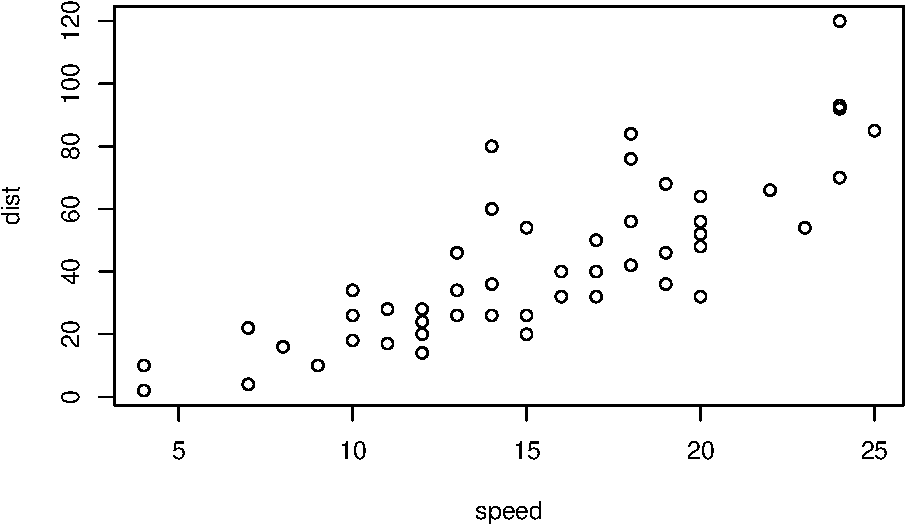
\includegraphics{PracticumNotebook_files/figure-latex/unnamed-chunk-1-1.pdf}

\begin{figure}
\centering
\includegraphics{https://zacw.rstudio.cloud/0469cf272cf741b183c40cf2932686cf/file_show?path=\%2Fcloud\%2Fproject\%2FBarChart_AgeRangeDistribution.png}
\caption{BarChart\_AgeRangeDistribution}
\end{figure}

\end{document}
